\section{From extracted surface to NURBS representation}
As of yet, there is no open-source software which provides the conversion from a \textit{mesh-based} geometry to NURBS representation. Hence, one of the main challenges of both the algorithmic and implementation part of this project is to develop one from scratch. Due to a variety of possible approaches to tackle this problem (e.g. \cite{becker2011advanced},\cite{eck1996automatic}), we have conducted a profound prototyping work. In order to avoid a cumbersome and time-consuming implementation overheads during the prototyping phase, we have used MATLAB \cite{MATLAB}. Once the algorithms to be used are finalized, the prototypes are to be implemented using a non-proprietary language, such as Python or C++.\todointern{this will be edited, of course.}
\subsection{Fitting pipeline}
\todointern[inline]{clean this up so this fits into implementation}
\begin{figure}
\centering
  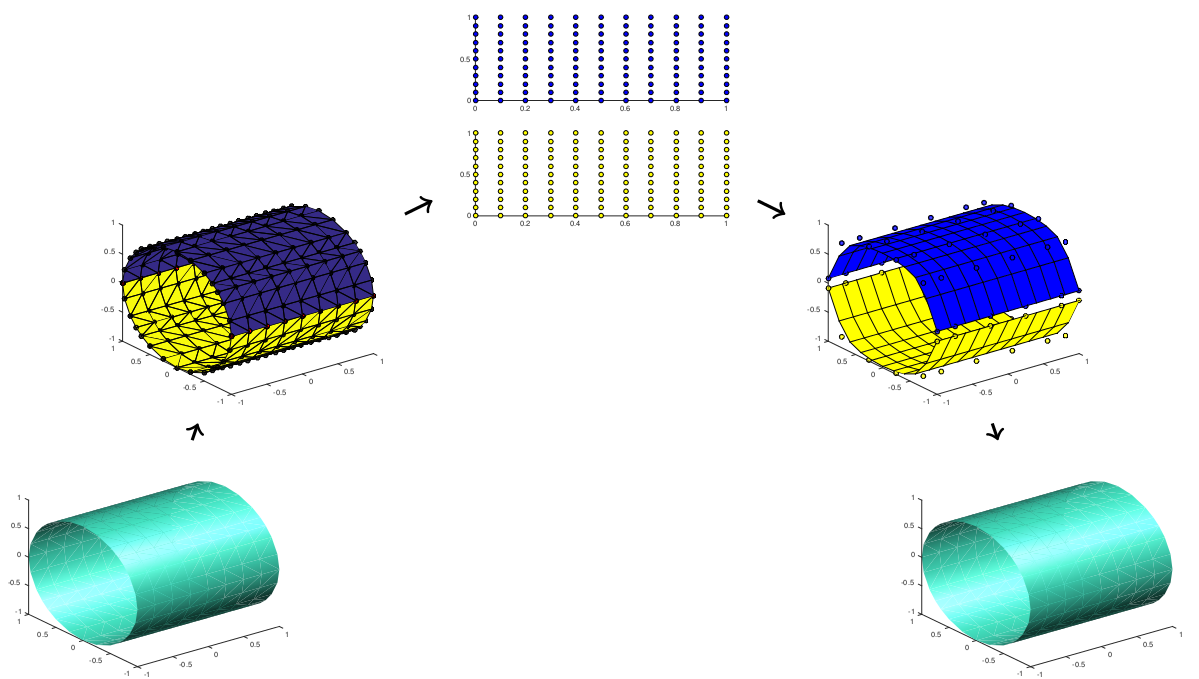
\includegraphics[width=.85\linewidth]{Fitting_workflow.png}
  \caption{NURBS fitting pipeline}
  \label{fig:fitting_pipeline}
\end{figure}
Since the geometry obtained after topology optimization can be arbitrary complex, we might not be able to find a good fit using only one patch. We seek a multi step algorithm, allowing us to break the overall big problem into smaller problems, which can be handled relatively easy.
Based on the algorithm described in \cite{eck1996automatic}, our overall fitting pipeline looks as follows (see \autoref{fig:fitting_pipeline}):
\begin{itemize}
	\item Patch selection (breaking our problem in small pieces which can be solved using least squares)
	\item Parametrization of obtained patches
	\item B-spline fitting using least squares
	\item Smooth connection of patches
	\item Conversion back to CAD
\end{itemize}

The pipeline given above, once implemented, will provide us with a flexible algorithm for converting an arbitrary complex mesh based geometry into NURBS and, hence, CAD-representation.
\subsection{Applying Peters' Scheme}
Following the example of using Peters' scheme to fit NURBS smoothly to datapoints in \cite{eck1996automatic}, we did extensive prototyping to ensure the tractability of using Peters' scheme (see \autoref{subsec:peters}) for fitting a NURBS surface (see \autoref{subsub:petersleastsq}) in our settings. As mentioned above, these prototypes were done in MATLAB, and were also partly implemented in Python. 

Among our prototypes we have:
\begin{itemize}
\item A Doo-Sabin subdivision scheme implemented in Python, which we use to organize the twice refined mesh in structures, from which you can extract the locality and neighbour information necessary to calculate the \Bez point coefficients on them in Peters' scheme
\item Implementations of the algorithm to calculate these \Bez point coefficients, as well as plotting them for debugging and visualisation
\item \Bez curve and surface evaluation via calculating the coefficients on each \Bez control point from a set of parameters
\item Algorithms to extract the necessary datapoints and parameters from the result data of the \acf{DC} algorithm in \autoref{ssec:DC}, using geometric conversions where necessary, and ignoring unusual datapoints
\item An algorithm for using the four above algorithms to assemble the total coefficient matrix in \autoref{eqn:petersminimisation} in \autoref{subsub:petersleastsq}
\item An application of MATLAB's built-in least squares minimisation tool to fit the resulting network of \Bez patches to the extracted surface.
\end{itemize}
A sample result, the fitting of a surface to a toroidal shape defined implicitly for the \acs{DC} algorithm is shown in \autoref{fig:fittingStructures}.

%In this section we will describe:
%\begin{itemize}
%\item That we apply the theory in section \autoref{subsec:peters} and \autoref{subsub:petersleastsq} about Peters' Scheme to fit datapoints from Dual Contouring in \autoref{ssec:DC} \tododone{fix this ref} and the coarse quads and the parameters on them to obtain a $G^1$ surface
%\item That we implemented this as Python classes and structures after MATLAB prototyping, \autoref{fig:fittingStructures} for reference
%\item How they work algorithmically, \textit{(whenever they work)}
%\item What libraries we used to do the least-squares an plotting an stuff
%\end{itemize}

\begin{figure}
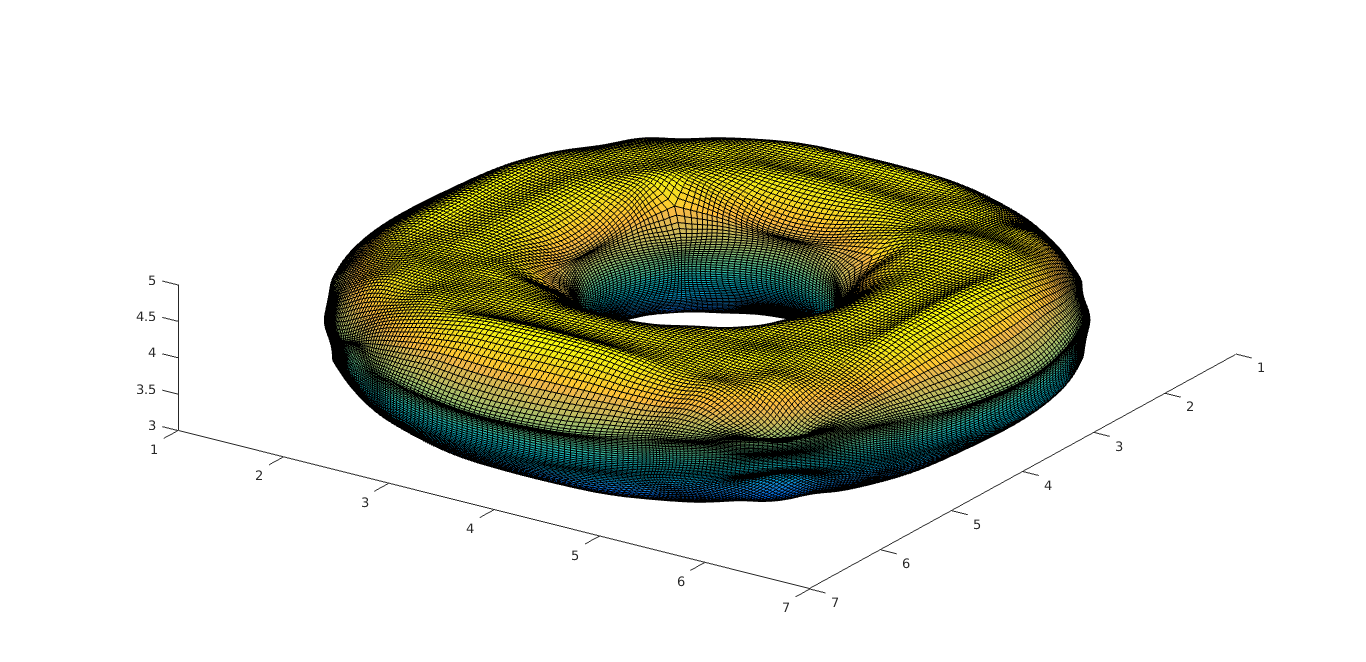
\includegraphics[width = \textwidth]{Pictures/NURBS/torus_from_DC.png}
\caption{A sample result from the Peters' scheme least-squares minimisation surface fitting, using the data provided by the \acs{DC} algorithm for an implicit function describing a torus. The grid lines on the figure are following the constant lines of each parameter value. As they follow the patch edges, corners where other than 4 coarse quads are meeting can be recognized, as for example on the middle of the far side of the torus, on the side that's facing the viewer.}
\label{fig:fittingStructures}
\end{figure}


